% Options for packages loaded elsewhere
\PassOptionsToPackage{unicode}{hyperref}
\PassOptionsToPackage{hyphens}{url}
\PassOptionsToPackage{dvipsnames,svgnames,x11names}{xcolor}
%
\documentclass[
]{article}
\usepackage{amsmath,amssymb}
\usepackage{lmodern}
\usepackage{iftex}
\ifPDFTeX
  \usepackage[T1]{fontenc}
  \usepackage[utf8]{inputenc}
  \usepackage{textcomp} % provide euro and other symbols
\else % if luatex or xetex
  \usepackage{unicode-math}
  \defaultfontfeatures{Scale=MatchLowercase}
  \defaultfontfeatures[\rmfamily]{Ligatures=TeX,Scale=1}
\fi
% Use upquote if available, for straight quotes in verbatim environments
\IfFileExists{upquote.sty}{\usepackage{upquote}}{}
\IfFileExists{microtype.sty}{% use microtype if available
  \usepackage[]{microtype}
  \UseMicrotypeSet[protrusion]{basicmath} % disable protrusion for tt fonts
}{}
\makeatletter
\@ifundefined{KOMAClassName}{% if non-KOMA class
  \IfFileExists{parskip.sty}{%
    \usepackage{parskip}
  }{% else
    \setlength{\parindent}{0pt}
    \setlength{\parskip}{6pt plus 2pt minus 1pt}}
}{% if KOMA class
  \KOMAoptions{parskip=half}}
\makeatother
\usepackage{xcolor}
\usepackage[margin=1in]{geometry}
\usepackage{color}
\usepackage{fancyvrb}
\newcommand{\VerbBar}{|}
\newcommand{\VERB}{\Verb[commandchars=\\\{\}]}
\DefineVerbatimEnvironment{Highlighting}{Verbatim}{commandchars=\\\{\}}
% Add ',fontsize=\small' for more characters per line
\usepackage{framed}
\definecolor{shadecolor}{RGB}{248,248,248}
\newenvironment{Shaded}{\begin{snugshade}}{\end{snugshade}}
\newcommand{\AlertTok}[1]{\textcolor[rgb]{0.94,0.16,0.16}{#1}}
\newcommand{\AnnotationTok}[1]{\textcolor[rgb]{0.56,0.35,0.01}{\textbf{\textit{#1}}}}
\newcommand{\AttributeTok}[1]{\textcolor[rgb]{0.77,0.63,0.00}{#1}}
\newcommand{\BaseNTok}[1]{\textcolor[rgb]{0.00,0.00,0.81}{#1}}
\newcommand{\BuiltInTok}[1]{#1}
\newcommand{\CharTok}[1]{\textcolor[rgb]{0.31,0.60,0.02}{#1}}
\newcommand{\CommentTok}[1]{\textcolor[rgb]{0.56,0.35,0.01}{\textit{#1}}}
\newcommand{\CommentVarTok}[1]{\textcolor[rgb]{0.56,0.35,0.01}{\textbf{\textit{#1}}}}
\newcommand{\ConstantTok}[1]{\textcolor[rgb]{0.00,0.00,0.00}{#1}}
\newcommand{\ControlFlowTok}[1]{\textcolor[rgb]{0.13,0.29,0.53}{\textbf{#1}}}
\newcommand{\DataTypeTok}[1]{\textcolor[rgb]{0.13,0.29,0.53}{#1}}
\newcommand{\DecValTok}[1]{\textcolor[rgb]{0.00,0.00,0.81}{#1}}
\newcommand{\DocumentationTok}[1]{\textcolor[rgb]{0.56,0.35,0.01}{\textbf{\textit{#1}}}}
\newcommand{\ErrorTok}[1]{\textcolor[rgb]{0.64,0.00,0.00}{\textbf{#1}}}
\newcommand{\ExtensionTok}[1]{#1}
\newcommand{\FloatTok}[1]{\textcolor[rgb]{0.00,0.00,0.81}{#1}}
\newcommand{\FunctionTok}[1]{\textcolor[rgb]{0.00,0.00,0.00}{#1}}
\newcommand{\ImportTok}[1]{#1}
\newcommand{\InformationTok}[1]{\textcolor[rgb]{0.56,0.35,0.01}{\textbf{\textit{#1}}}}
\newcommand{\KeywordTok}[1]{\textcolor[rgb]{0.13,0.29,0.53}{\textbf{#1}}}
\newcommand{\NormalTok}[1]{#1}
\newcommand{\OperatorTok}[1]{\textcolor[rgb]{0.81,0.36,0.00}{\textbf{#1}}}
\newcommand{\OtherTok}[1]{\textcolor[rgb]{0.56,0.35,0.01}{#1}}
\newcommand{\PreprocessorTok}[1]{\textcolor[rgb]{0.56,0.35,0.01}{\textit{#1}}}
\newcommand{\RegionMarkerTok}[1]{#1}
\newcommand{\SpecialCharTok}[1]{\textcolor[rgb]{0.00,0.00,0.00}{#1}}
\newcommand{\SpecialStringTok}[1]{\textcolor[rgb]{0.31,0.60,0.02}{#1}}
\newcommand{\StringTok}[1]{\textcolor[rgb]{0.31,0.60,0.02}{#1}}
\newcommand{\VariableTok}[1]{\textcolor[rgb]{0.00,0.00,0.00}{#1}}
\newcommand{\VerbatimStringTok}[1]{\textcolor[rgb]{0.31,0.60,0.02}{#1}}
\newcommand{\WarningTok}[1]{\textcolor[rgb]{0.56,0.35,0.01}{\textbf{\textit{#1}}}}
\usepackage{longtable,booktabs,array}
\usepackage{calc} % for calculating minipage widths
% Correct order of tables after \paragraph or \subparagraph
\usepackage{etoolbox}
\makeatletter
\patchcmd\longtable{\par}{\if@noskipsec\mbox{}\fi\par}{}{}
\makeatother
% Allow footnotes in longtable head/foot
\IfFileExists{footnotehyper.sty}{\usepackage{footnotehyper}}{\usepackage{footnote}}
\makesavenoteenv{longtable}
\usepackage{graphicx}
\makeatletter
\def\maxwidth{\ifdim\Gin@nat@width>\linewidth\linewidth\else\Gin@nat@width\fi}
\def\maxheight{\ifdim\Gin@nat@height>\textheight\textheight\else\Gin@nat@height\fi}
\makeatother
% Scale images if necessary, so that they will not overflow the page
% margins by default, and it is still possible to overwrite the defaults
% using explicit options in \includegraphics[width, height, ...]{}
\setkeys{Gin}{width=\maxwidth,height=\maxheight,keepaspectratio}
% Set default figure placement to htbp
\makeatletter
\def\fps@figure{htbp}
\makeatother
\setlength{\emergencystretch}{3em} % prevent overfull lines
\providecommand{\tightlist}{%
  \setlength{\itemsep}{0pt}\setlength{\parskip}{0pt}}
\setcounter{secnumdepth}{5}
\usepackage{amssymb}
\usepackage{booktabs}
\usepackage{longtable}
\usepackage{array}
\usepackage{multirow}
\usepackage{wrapfig}
\usepackage{float}
\usepackage{colortbl}
\usepackage{pdflscape}
\usepackage{tabu}
\usepackage{threeparttable}
\usepackage{threeparttablex}
\usepackage[normalem]{ulem}
\usepackage{makecell}
\usepackage{xcolor}
\ifLuaTeX
  \usepackage{selnolig}  % disable illegal ligatures
\fi
\IfFileExists{bookmark.sty}{\usepackage{bookmark}}{\usepackage{hyperref}}
\IfFileExists{xurl.sty}{\usepackage{xurl}}{} % add URL line breaks if available
\urlstyle{same} % disable monospaced font for URLs
\hypersetup{
  pdftitle={Final\_project\_Bottino\_Poetto\_Spagliardi},
  pdfauthor={Manuel Bottino, Patrick Poetto, Jacopo Spagliardi},
  colorlinks=true,
  linkcolor={Maroon},
  filecolor={Maroon},
  citecolor={Blue},
  urlcolor={blue},
  pdfcreator={LaTeX via pandoc}}

\title{Final\_project\_Bottino\_Poetto\_Spagliardi}
\author{Manuel Bottino, Patrick Poetto, Jacopo Spagliardi}
\date{2023-06-17}

\begin{document}
\maketitle

{
\hypersetup{linkcolor=}
\setcounter{tocdepth}{2}
\tableofcontents
}
\hypertarget{references}{%
\section{References}\label{references}}

{[}1{]} C. M. Bishop. \emph{Pattern Recognition and Machine Learning}.
Ed. by M. Jordan. Information Science and Statistics. Springer, 2006.

{[}2{]} L. Breiman. ``Bagging predictions''. In: \emph{Machine Learning}
24.2 (1996), pp.~123-140.

{[}3{]} e. a. Han Jiawei. \emph{Data Mining Concepts and Techniques}.
Morgan Kaufmann Publishers, 2023.

{[}4{]} e. a. Hastie Trevor. \emph{The Elements of Statistical
Learning}. Vol. 27. 2. 2009. Chap. 9, p.~745.

{[}5{]} e. a. Kuhn Max. \emph{Applied Predictive Modeling}. Springer,
2016.

{[}6{]} e. a. Seni Giovanni. \emph{Ensemble Methods in Data Mining:
Improving Accuracy Through Combining Predictions}. Ed. by C. Robert
Grossman University of Illinois. Synthesis Lectures on Data Mining and
Knowledge Discovery. Morgan\&Claypool Publishers, 2010.

\newpage

\hypertarget{review}{%
\section{Review}\label{review}}

The underlying idea of bagging is to create multiple instances of the
base model (e.g., a decision tree) trained on randomly selected samples
of data with replacement (bootstrapping, that's why this technique is
also called Bootstrap aggregating). Each base model is trained on
subsets of the original data, independently of the others, producing a
prediction. The predictions of the individual models are then combined
using a majority voting rule (for classification problems) or averaging
(for regression problems) to obtain a final prediction. By creating
different instances of the base model and combining their predictions,
bagging can reduce variability and improve overall predictive
performance. Let's see how this type of ensemble technique works:

\begin{itemize}
    \item Divide our dataset randomly into two different groups of rows: 
    \begin{itemize}
        \item Training Data: the larger part of our group that will be used to produce new datasets.
        \item Testing Data: the smaller part that will be used to see the performance of our technique.
    \end{itemize}
    \item Produce with bootstrap technique new datasets using Training Data. Each bootstrap sample is created by randomly selecting with replacement from the original sample. This means that some rows may be selected multiple times, while others may be excluded to reach the dimension of the original sample. It produced a number $N$ of samples
    \item Using each sample we produce $N$ models (always the same type of model, for example, linear regression model) that we can call $M_k$ with $k={1, ..., N}$
    \item Then we can use each model to produce predictions using Testing Data.
    \item Assembling all the predictions in a democratic way if the variable we are predicting is categorical, and in an averaging way if the variable is continuous
    \item This assembled prediction is more accurate than the prediction made by the same model but create only uses the original dataset.
\end{itemize}

\begin{center}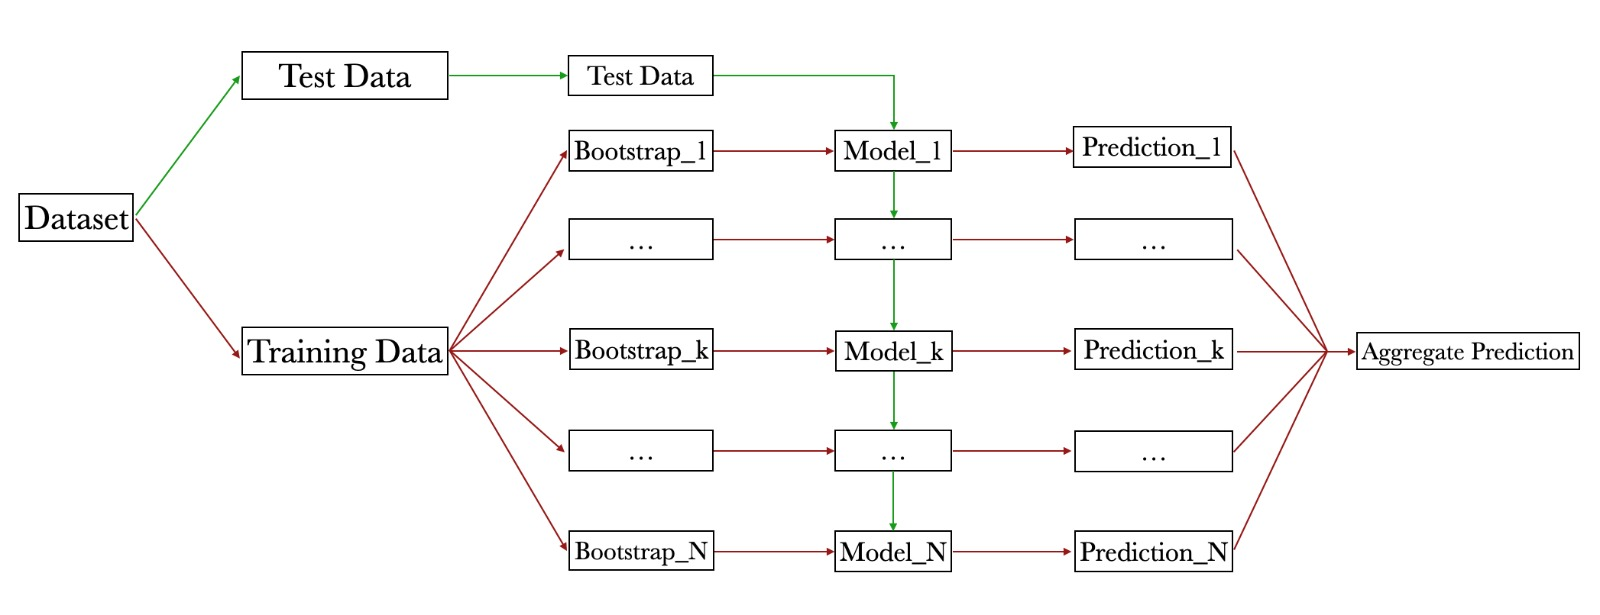
\includegraphics[width=1\linewidth]{Immagine WhatsApp 2023-06-16 ore 14.20.18} \end{center}

\hypertarget{why-it-works}{%
\subsection{Why it works}\label{why-it-works}}

First of all let's introduce the general idea of bagging. Given a
dataset \(L=\{(x_n,y_n),\ n=1, \ldots ,N\}\) we try to improve a
predicting procedure in a ``naive'' way, ideally we would like to have a
sequence of datasets \(\{L_k\}\) each containing N independent
observations, then take the average of the sequence
\(\{\phi(x, L_k)\}\).

\begin{equation}
\phi_A(x,P)=E_L[\phi(x,L)]\label{eq:agg}
\end{equation}

Because \(\phi_A\) depends not only on x but also the underlying
probability distribution \(P\) from which L is drawn. Since we are
missing this last information the only tool we are left with is our
dataset L, we instead use \(P_L\) the bootstrap approximation of \(P\),
it can be defined as the probability mass function with equal
probability of extracting each element of the dataset \((x_n,y_n)\).
Finally we can define the bootstrap aggregate predictor as:

\begin{equation}
\phi_B (x)=\phi_A(x,P_L)\label{eq:boot}
\end{equation}

In order to understand why bagging works theoretically it can be proved
that mean-squared error (MSE) of \(\phi_A(x)\) is lower than the
mean-squared error averaged over L of \(\phi(x,L)\). How much lower the
two sides are depends on the inequality:

\begin{equation}
[E_L\phi(x,L)]^2\leq E_L\phi^2(x,L)\label{eq:ineq}
\end{equation}

This result is true taking advantage of the Jensen's inequality for the
specific case in which \(g(X)=X^2\), this function is convex
(\(g''>0\)), thus \(E[Z^2] \geq (E[Z])^2\)

\hypertarget{instability}{%
\subsection{Instability}\label{instability}}

The inequality \ref{eq:ineq} is a nice starting point to explain what
role instability plays. In fact, If \(\phi(x, L)\) does not change too
much with replicate L the two sides will be nearly equal, and
aggregation will not help. The more highly variable the \(\phi(x, L)\)
are, the more improvement aggregation may produce. Applying this
reasoning to our \(\phi_B (x)\), if the procedure is unstable, it can
give improvement through aggregation. However, if the procedure is
stable, then \(\phi_B (x)=\phi_A(x,P_L)\) will not be as accurate for
data drawn from \(P\) as \(\phi_A(X, P) \sim \phi(x,L)\).

Let's see how this concept can be translated when we look at a more
specific context, like classification. In this instance the predictor
\(\phi(\pmb x,L)\) predicts a label \(j \in \{1,..., J\}\). We first
define \(Q(j|x)=P(\phi(x,L)=j)\), over many independent replicates of
the learning set \(L\), \(\phi\) predicts class label \(j\) at input
\(x\) with relative frequency \(Q(j|x)\), and let \(P(j|x)\) be the
probability that input x generates class \(j\). At this point we can set
\(\phi^*(x)= \arg \max _j P(j|x)\) (the Bayes predictor) which leads to
the following expression for \(Q (j |x)\):

\[
\begin{cases}
1 \ if \ P(j|x)=max_iP(i|x) \\
0 \ elsewhere
\end{cases}
\]

Now we have all the ingredients to show the maximum classification rate
for: \begin{equation}
r^*=\int \max_j P(j|x) P_X(dx)\label{eq:class_max}
\end{equation}

where \(P_X(dx)\) is the probability distribution of X.

Also, call \(\phi\) order-correct at the input \(\pmb x\) if:
\begin{equation}
\arg \max_j Q(j|x)=\arg \max_j P(j|x)=\label{eq:ord_corr}
\end{equation}

If we now focus on the aggregate of \(\phi\) and define it following the
procedure described above \(\phi_A(x)=\arg \max_j Q(j|x)\). We have the
maximum attainable correct-classification rate (accuracy) of
\(\phi(x)\), we are missing the corret-classification for x, which for
\(\phi_A(x)\) is \(\sum_j I(\arg \max_j Q(j|x)=j)P(j|x)\) Where \(I\) is
the indicator function.

\emph{Putting all the pieces together} the correct-classification rate
for \(\phi_A(x)\) is: \begin{equation}
r_A=\int_{\pmb x \in C} max_j P(j| \pmb x) P_X(d \pmb x)+ \int_{\pmb x \in C’} [\sum_j(I(\phi_A(\pmb x)=j)P(j|\pmb x)] P_X(\pmb x)
\label{eq:class_res}
\end{equation} Even if \(\phi\) is order correct at \(x\) its correct
classification rate can be far from optimal, but \(\phi_A\) is optimal.
Only if \(\phi\) is order-correct for most input of x (it is good), then
aggregation can transform it into a nearly optimal predictor. On the
other hand, unlike the numerical prediction situation, poor predictors
can be transformed into worse ones if we use bagging.

\hypertarget{model---decision-tree-based-methods}{%
\subsection{Model - Decision Tree-Based
Methods}\label{model---decision-tree-based-methods}}

Tree-based methods partition the feature space into a set of rectangles,
and then fit a simple model, say a constant, in each one. This is a
simple yet powerful procedure since it is able to disentangle a model
into simpler and smaller models and describe his features more
accurately than global models do basically using binary conditional
clustering. The geometric perspective described before can be seen as a
tree where data are run and at each node a test is conducted to see what
is the path a covariate should follow until reaching a leaf, which
represents the final prediction explained by the constant model. For
example, let's say we have \(p\) inputs and a response, for each of
\(N\) observations: that is, \((x_i,y_i)\) for \(i = 1,2,...,N\), with
\(x_i = (x_{i1},x_{i2},...,x_{ip})\). The algorithm has decide on the
splitting variables and split points, as well as what shape the tree
should have. Suppose first that we have a partition into \(M\) regions
\(R_1, R_2, ..., R_M\), and we model the response as a constant \(c_m\)
in each region: As a criterion for optimal partitional we can minimize
the sum of squares \(\sum(y_i-f(x_i))^2\). In this way the best
\(\hat{c}_m\) is just the average of \(y_i\) in region \(R_m\):
\(\hat{c}_m=av(y_i | x_i \in R_m)\). Our model will be then:
\(f(x)=\sum_{m=1}^{M} c_m \cdot I(x \in R_m)\).

Now finding the best binary partition in terms of minimum sum of squares
is generally computationally infeasible so we can set up a CART
(classification and regression tree) algorithm starting with the data, a
splitting variable \(j\), a split point \(s\), and defining the half
planes as: \(R_1(j,s) = \{X\mid X_j \leq s\}\) and
\(R_2(j,s) = \{X\mid X_j > s\}\). Then we seek \(j\) and \(s\) that
solve

\begin{center}
$\underset{j,s}{\min}\left[\underset{c_1}{\min}\sum_{x_i \in R_1(j,s)} (y_i-c_1)^2 + \underset{c_2}{\min} \sum_{x_i \in R_2(j,s)} (y_i-c_2)^2\right]$
\end{center}

For any choice \(j\) and \(s\), the inner minimization is solved by:

\begin{center}
$\hat{c}_1 = \text{av}(y_i \,|\, x_i \in R_1(j, s)) \quad \text{and} \quad \hat{c}_2 = \text{av}(y_i \,|\, x_i \in R_2(j, s))$
\end{center}

For each \(j\), the split point \(s\) can be found very quickly and
hence determination of the best pair (j, s) is feasible by brute force.
Having found the best split, we partition the data into the two
resulting regions and repeat the splitting process on each of the two
regions. Then this process is repeated on all of the resulting regions.
The question now become: how large should we grow the tree? It is pretty
straightforward that too many nodes (splits) may overfit the data while
doing vice versa may end up not being able to capture them well,
resulting in misprediction. One strategy could be to set a lower
threshold for the decrease of the sum of squares and stop the splitting
when this is reached. However this strategy is too short sighted since a
seemingly worthless split may lead to a very good one below. A more
robust strategy may be to do kind of the opposite: grow a very large
tree and then use a cost-complexity pruning criterion to collapse one
internal node at a time from the full tree until the single node tree so
that we find a sequence. It is intuitive that the optimal tree must be
somewhere in the sequence. Now, with a cross validation selection
method, we can find the actual optimal tree just minimizing the cross
validated sum of squares.

This is how the CART algorithm for growing decision trees basically
works. Note that decision trees are divided in classification and
regression trees if the response is a factor or a numerical or continous
variable.

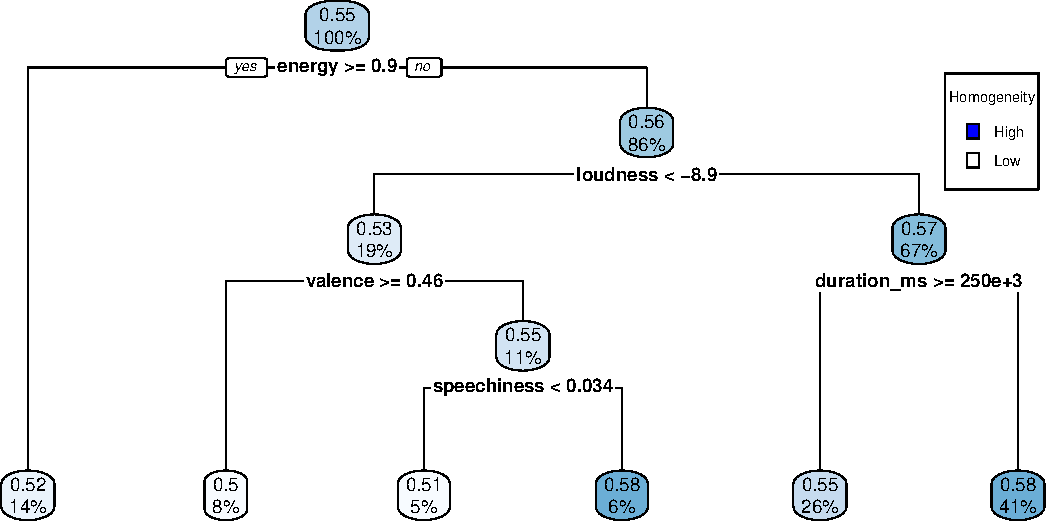
\includegraphics{Final_project_Bottino_Poetto_Spagliardi_files/figure-latex/unnamed-chunk-5-1.pdf}

\begin{longtable}[]{@{}ll@{}}
\toprule()
Predicted Value & Median Value \\
\midrule()
\endhead
0.5845508 & 0.55 \\
\bottomrule()
\end{longtable}

We used the well known Spotify dataset to grow a basic tree with the
function ``rpart''. The thresholds at each node are defined by the
algorithm which minimizes the MSE of the model. The color of each nodes
represent homogeneity across data which have been classified in a node.
Each node show the percentage of observations that it contains and the
outcome prediction for that node. Then we used the function ``predict''
applied to our grown tree to make prediction on a virtual new
observation, providing the median of each variable as a new value and
getting predicted popularity of a song which have the median as each
feature available in the dataset. Not surprisingly, the predicted value
for popularity is near the median of the covariate popularity itself.

\hypertarget{algorithm-setup}{%
\subsection{Algorithm Setup}\label{algorithm-setup}}

Bootstrap aggregating Regression Trees can be done following the
procedure proposed by \textbf{(Breiman, 1996)}:

\begin{enumerate}
\def\labelenumi{\arabic{enumi}.}
\item
  Randomly divide a real dataset into a \(10\%\) test \(\mathcal{T}\)
  and a \(90\%\) learning set \(\mathcal{L}\). If the dataset is
  simulated then we can consider a \(15-85\) or a \(20-80\) proportion.
\item
  Grow a regression tree from \(\mathcal{L}\) using a 10-fold cross
  validation, then run \(\mathcal{T}\) down the tree to obtain the
  squared error \(e_S(L, T)\). Using che k-folds cross validation means
  that \(\mathcal{L}\) is divided into \(10\) folds, and for each
  iteration, a regression tree is trained on \(9\) folds and evaluated
  on the remaining fold. The process is repeated \(10\) times, such that
  each fold is utilized as the test set once. Ultimately, the best
  model, i.e.~the regression tree with the best average performance
  across all test folds, is selected as the final result. At the end of
  the \(10\) iterations, the squared errors obtained for each test fold
  are used to calculate the mean squared error \(e_S(L, T)\), which
  represents the average squared difference between the predictions of
  the regression tree and the actual values of the test set.
\item
  Select a bootstrap sample \(\mathcal{L}_B\) from \(\mathcal{L}\) and
  use it to grow a tree. Then use \(\mathcal{L}\) to prune the tree
  avoiding overfitting. Repeat this step \(25\) times to obtain
  predictors \(\phi_1(\mathbf{x}), ..., \phi_{25}(\mathbf{x})\).
\item
  For \((y_n,\mathbf{x_n}) \in \mathcal{T}\), the bagged predictor will
  be \(\hat{y}_n = av_k\phi_k(\mathbf{x_n})\), and the squared error
  \(e_B(\mathcal{L,T})= av_n(y_n - \hat{y}_n)^2\).
\item
  Divide the data into \(\mathcal{L}\) and \(\mathcal{T}\) for \(100\)
  times and average the errors to obtain \(\bar{e}_S\) and
  \(\bar{e}_B\).
\end{enumerate}

\hypertarget{application-of-algorithm}{%
\subsection{Application of algorithm}\label{application-of-algorithm}}

Try to replicate the algorithm provided by the paper for regression
trees using 10-fold cross-validation and bagging

\begin{Shaded}
\begin{Highlighting}[]
\FunctionTok{set.seed}\NormalTok{(}\DecValTok{655}\NormalTok{)}
\CommentTok{\# Function that randomize learning and testing datasets, point 5 of algorithm}
\CommentTok{\# performs this 100 time. To each division the author applies both methods (cross }
\CommentTok{\# validation and bagging). }

\NormalTok{random\_training\_test}\OtherTok{=}\ControlFlowTok{function}\NormalTok{(df,k, }\AttributeTok{bin\_80\_20=}\DecValTok{0}\NormalTok{)\{}
\NormalTok{  fold\_indices }\OtherTok{\textless{}{-}} \FunctionTok{sample}\NormalTok{(}\FunctionTok{cut}\NormalTok{(}\FunctionTok{seq}\NormalTok{(}\DecValTok{1}\NormalTok{, }\FunctionTok{nrow}\NormalTok{(df)), }\AttributeTok{breaks =}\NormalTok{ k, }\AttributeTok{labels =} \ConstantTok{FALSE}\NormalTok{, }
                             \AttributeTok{ordered\_result =} \ConstantTok{FALSE}\NormalTok{))}
  \ControlFlowTok{if}\NormalTok{ (bin\_80\_20}\SpecialCharTok{==}\DecValTok{1}\NormalTok{) \{}
\NormalTok{    test\_indices }\OtherTok{\textless{}{-}} \FunctionTok{which}\NormalTok{(fold\_indices }\SpecialCharTok{==} \DecValTok{1} \SpecialCharTok{|}\NormalTok{ fold\_indices }\SpecialCharTok{==} \DecValTok{2}\NormalTok{)}
\NormalTok{  \}}\ControlFlowTok{else}\NormalTok{ \{}
\NormalTok{    test\_indices }\OtherTok{\textless{}{-}} \FunctionTok{which}\NormalTok{(fold\_indices }\SpecialCharTok{==} \DecValTok{1}\NormalTok{)\}}
  
\NormalTok{  train\_i }\OtherTok{\textless{}{-}}\NormalTok{ df[}\SpecialCharTok{{-}}\NormalTok{test\_indices, ]}
\NormalTok{  test\_i }\OtherTok{\textless{}{-}}\NormalTok{ df[test\_indices, ]}
  \FunctionTok{return}\NormalTok{(}\FunctionTok{list}\NormalTok{(train\_i,test\_i))}
\NormalTok{\}}



\NormalTok{k\_fold\_reg\_tree}\OtherTok{=} \ControlFlowTok{function}\NormalTok{(df,k, y)\{}
\NormalTok{  formula }\OtherTok{\textless{}{-}} \FunctionTok{as.formula}\NormalTok{(}\FunctionTok{paste}\NormalTok{(y, }\StringTok{"\textasciitilde{}"}\NormalTok{, }\StringTok{"."}\NormalTok{))}
  
  \CommentTok{\# 1. take the dataset and divide it into learning and testing (90\% {-} 10\%)}
  \CommentTok{\# which is already done by the function random\_training\_test}
\NormalTok{  train\_i}\OtherTok{=}\NormalTok{df[[}\DecValTok{1}\NormalTok{]]}
\NormalTok{  test\_i}\OtherTok{=}\NormalTok{df[[}\DecValTok{2}\NormalTok{]]}
  
  
  \CommentTok{\# 2. take the learning set and apply 10{-}fold cv to find the model with lowest MSE}
  
\NormalTok{  fold\_indices }\OtherTok{\textless{}{-}} \FunctionTok{sample}\NormalTok{(}\FunctionTok{cut}\NormalTok{(}\FunctionTok{seq}\NormalTok{(}\DecValTok{1}\NormalTok{, }\FunctionTok{nrow}\NormalTok{(train\_i)), }\AttributeTok{breaks =}\NormalTok{ k, }\AttributeTok{labels =} \ConstantTok{FALSE}\NormalTok{, }
                             \AttributeTok{ordered\_result =} \ConstantTok{FALSE}\NormalTok{) )}
  
\NormalTok{  cv\_result}\OtherTok{=}\ConstantTok{Inf}
  
  \ControlFlowTok{for}\NormalTok{ (i }\ControlFlowTok{in} \DecValTok{1}\SpecialCharTok{:}\NormalTok{k) \{}

  
  \CommentTok{\# Split the data into training and testing sets (10{-}fold cross validation)}
\NormalTok{  test\_indices }\OtherTok{\textless{}{-}} \FunctionTok{which}\NormalTok{(fold\_indices }\SpecialCharTok{==}\NormalTok{ i)}
\NormalTok{  train\_data }\OtherTok{\textless{}{-}}\NormalTok{ train\_i[}\SpecialCharTok{{-}}\NormalTok{test\_indices, ]}
\NormalTok{  test\_data }\OtherTok{\textless{}{-}}\NormalTok{ train\_i[test\_indices, ]}
  
  
  
  \CommentTok{\# Train a regression tree on the training set}
\NormalTok{  model }\OtherTok{\textless{}{-}} \FunctionTok{rpart}\NormalTok{(formula, }\AttributeTok{data =}\NormalTok{ train\_data)}
  
  \CommentTok{\# Predict the target variable for the testing set}
\NormalTok{  predictions }\OtherTok{\textless{}{-}} \FunctionTok{predict}\NormalTok{(model, }\AttributeTok{newdata =}\NormalTok{ test\_data)}
   
  
  \CommentTok{\#Calculate the evaluation metric (mean squared errors)}
\NormalTok{  result }\OtherTok{\textless{}{-}} \FunctionTok{mean}\NormalTok{((predictions }\SpecialCharTok{{-}}\NormalTok{ test\_data[[y]])}\SpecialCharTok{\^{}}\DecValTok{2}\NormalTok{)}
  \CommentTok{\# 3. For every candidate we compute the MSE compered to the original test}
  
  \ControlFlowTok{if}\NormalTok{(result}\SpecialCharTok{\textless{}}\NormalTok{cv\_result)\{}
\NormalTok{    cv\_result}\OtherTok{=}\NormalTok{result}
    \CommentTok{\# Compute mse of this model using the original test set as comparison}
\NormalTok{    predictions }\OtherTok{\textless{}{-}} \FunctionTok{predict}\NormalTok{(model, }\AttributeTok{newdata =}\NormalTok{ test\_i)}
\NormalTok{    final\_res}\OtherTok{=}\FunctionTok{mean}\NormalTok{((predictions }\SpecialCharTok{{-}}\NormalTok{ test\_i[[y]])}\SpecialCharTok{\^{}}\DecValTok{2}\NormalTok{)}
\NormalTok{  \}}
\NormalTok{  \}}
  \FunctionTok{return}\NormalTok{(final\_res)}
\NormalTok{\}}

\NormalTok{reg\_tree\_boot}\OtherTok{=} \ControlFlowTok{function}\NormalTok{(df,b, y)\{}
\NormalTok{  formula }\OtherTok{\textless{}{-}} \FunctionTok{as.formula}\NormalTok{(}\FunctionTok{paste}\NormalTok{(y, }\StringTok{"\textasciitilde{}"}\NormalTok{, }\StringTok{"."}\NormalTok{))}
  
  \CommentTok{\# 1. take the dataset and divide it into learning and testing (90\% {-} 10\%)}
  \CommentTok{\# which is already done by the function }
\NormalTok{  train\_i}\OtherTok{=}\NormalTok{df[[}\DecValTok{1}\NormalTok{]]}
\NormalTok{  test\_i}\OtherTok{=}\NormalTok{df[[}\DecValTok{2}\NormalTok{]]}
\NormalTok{  predictions}\OtherTok{=}\FunctionTok{rep}\NormalTok{(}\DecValTok{0}\NormalTok{, }\FunctionTok{nrow}\NormalTok{(test\_i))}
  
  \CommentTok{\# 2. compute 25 predictions with different bootstrap samples}
  \ControlFlowTok{for}\NormalTok{ (i }\ControlFlowTok{in} \DecValTok{1}\SpecialCharTok{:}\NormalTok{b) \{}
\NormalTok{  train\_data}\OtherTok{=}\FunctionTok{slice\_sample}\NormalTok{(train\_i,}\AttributeTok{n=}\FunctionTok{nrow}\NormalTok{(train\_i), }\AttributeTok{replace=}\ConstantTok{TRUE}\NormalTok{)}
\NormalTok{  model }\OtherTok{\textless{}{-}} \FunctionTok{rpart}\NormalTok{(formula, }\AttributeTok{data =}\NormalTok{ train\_data)}
  
  \CommentTok{\# point three of the algorithm is also about pruned trees using the original }
  \CommentTok{\# training set. the function prune determines a nested sequence of subtrees }
  \CommentTok{\# of the supplied rpart object by recursively snipping off the least important splits, }
  \CommentTok{\# based on the complexity parameter (cp).}
\NormalTok{  pruned\_tree }\OtherTok{\textless{}{-}}\NormalTok{ rpart}\SpecialCharTok{::}\FunctionTok{prune}\NormalTok{(model, }\AttributeTok{cp=}\FloatTok{0.01}\NormalTok{, }\AttributeTok{newdata=}\NormalTok{train\_i)}
  
  \CommentTok{\# Predict the target variable for the testing set}
\NormalTok{  predictions }\OtherTok{\textless{}{-}}\NormalTok{ predictions }\SpecialCharTok{+} \FunctionTok{predict}\NormalTok{(pruned\_tree, }\AttributeTok{newdata =}\NormalTok{ test\_i)}
   
\NormalTok{  \}}
  \CommentTok{\# 3. take the mean of these predictors and compute the MSE}
\NormalTok{  predictions}\OtherTok{\textless{}{-}}\NormalTok{predictions}\SpecialCharTok{/}\NormalTok{b}
\NormalTok{  final\_res}\OtherTok{=}\FunctionTok{mean}\NormalTok{((predictions }\SpecialCharTok{{-}}\NormalTok{ test\_i[[y]])}\SpecialCharTok{\^{}}\DecValTok{2}\NormalTok{)}
  \FunctionTok{return}\NormalTok{(final\_res)}
\NormalTok{\}}

\CommentTok{\# I wrote down y instead of the standard MEDV (median of prices) so my lapply below}
\CommentTok{\# can be computed}
\NormalTok{housing }\OtherTok{\textless{}{-}} \FunctionTok{read.table}\NormalTok{(}\StringTok{"housing.csv"}\NormalTok{, }\AttributeTok{quote=}\StringTok{"}\SpecialCharTok{\textbackslash{}"}\StringTok{"}\NormalTok{, }\AttributeTok{comment.char=}\StringTok{""}\NormalTok{)}
\FunctionTok{colnames}\NormalTok{(housing)}\OtherTok{=}\FunctionTok{c}\NormalTok{(}\StringTok{\textquotesingle{}CRIM\textquotesingle{}}\NormalTok{, }\StringTok{\textquotesingle{}ZN\textquotesingle{}}\NormalTok{, }\StringTok{\textquotesingle{}INDUS\textquotesingle{}}\NormalTok{, }\StringTok{\textquotesingle{}CHAS\textquotesingle{}}\NormalTok{, }\StringTok{\textquotesingle{}NOX\textquotesingle{}}\NormalTok{, }\StringTok{\textquotesingle{}RM\textquotesingle{}}\NormalTok{, }\StringTok{\textquotesingle{}AGE\textquotesingle{}}\NormalTok{, }\StringTok{\textquotesingle{}DIS\textquotesingle{}}\NormalTok{,}
                    \StringTok{\textquotesingle{}RAD\textquotesingle{}}\NormalTok{, }\StringTok{\textquotesingle{}TAX\textquotesingle{}}\NormalTok{, }\StringTok{\textquotesingle{}PTRATIO\textquotesingle{}}\NormalTok{, }\StringTok{\textquotesingle{}B\textquotesingle{}}\NormalTok{, }\StringTok{\textquotesingle{}LSTAT\textquotesingle{}}\NormalTok{, }\StringTok{\textquotesingle{}y\textquotesingle{}}\NormalTok{)}

\CommentTok{\# I wrote down y instead of the standard O3 (ozone levels) so my lapply below}
\CommentTok{\# can be computed}
\FunctionTok{colnames}\NormalTok{(ozone)[}\DecValTok{1}\NormalTok{]}\OtherTok{=}\StringTok{"y"}

\NormalTok{B}\OtherTok{=}\DecValTok{1000}

\NormalTok{friedman1}\OtherTok{=}\FunctionTok{t}\NormalTok{(}\FunctionTok{replicate}\NormalTok{(B, \{}
\NormalTok{  fried1}\OtherTok{=}\FunctionTok{mlbench.friedman1}\NormalTok{(}\AttributeTok{n=}\DecValTok{1200}\NormalTok{, }\AttributeTok{sd=}\DecValTok{1}\NormalTok{)}
  \FunctionTok{data.frame}\NormalTok{(}\FunctionTok{cbind}\NormalTok{(fried1}\SpecialCharTok{$}\NormalTok{x,fried1}\SpecialCharTok{$}\NormalTok{y))\}}
\NormalTok{  ))}
\FunctionTok{colnames}\NormalTok{(friedman1)}\OtherTok{=}\FunctionTok{c}\NormalTok{(}\StringTok{"x\_1"}\NormalTok{,}\StringTok{"x\_2"}\NormalTok{,}\StringTok{"x\_3"}\NormalTok{,}\StringTok{"x\_4"}\NormalTok{,}\StringTok{"x\_5"}\NormalTok{,}\StringTok{"x\_6"}\NormalTok{,}\StringTok{"x\_7"}\NormalTok{,}\StringTok{"x\_8"}\NormalTok{,}\StringTok{"x\_9"}\NormalTok{,}\StringTok{"x\_10"}\NormalTok{,}\StringTok{"y"}\NormalTok{)}

\NormalTok{friedman2}\OtherTok{=}\FunctionTok{t}\NormalTok{(}\FunctionTok{replicate}\NormalTok{(B, \{}
\NormalTok{  fried2 }\OtherTok{\textless{}{-}} \FunctionTok{mlbench.friedman2}\NormalTok{(}\AttributeTok{n =} \DecValTok{1200}\NormalTok{)}
  \FunctionTok{data.frame}\NormalTok{(}\FunctionTok{cbind}\NormalTok{(fried2}\SpecialCharTok{$}\NormalTok{x,fried2}\SpecialCharTok{$}\NormalTok{y))\}}
\NormalTok{  ))}
\FunctionTok{colnames}\NormalTok{(friedman2)}\OtherTok{=}\FunctionTok{c}\NormalTok{(}\StringTok{"x\_1"}\NormalTok{,}\StringTok{"x\_2"}\NormalTok{,}\StringTok{"x\_3"}\NormalTok{,}\StringTok{"x\_4"}\NormalTok{,}\StringTok{"y"}\NormalTok{)}

\NormalTok{friedman3}\OtherTok{=}\FunctionTok{t}\NormalTok{(}\FunctionTok{replicate}\NormalTok{(B, \{}
\NormalTok{  fried3 }\OtherTok{\textless{}{-}} \FunctionTok{mlbench.friedman3}\NormalTok{(}\AttributeTok{n =} \DecValTok{1200}\NormalTok{)}
  \FunctionTok{data.frame}\NormalTok{(}\FunctionTok{cbind}\NormalTok{(fried3}\SpecialCharTok{$}\NormalTok{x,fried3}\SpecialCharTok{$}\NormalTok{y))\}}
\NormalTok{  ))}
\FunctionTok{colnames}\NormalTok{(friedman3)}\OtherTok{=}\FunctionTok{c}\NormalTok{(}\StringTok{"x\_1"}\NormalTok{,}\StringTok{"x\_2"}\NormalTok{,}\StringTok{"x\_3"}\NormalTok{,}\StringTok{"x\_4"}\NormalTok{,}\StringTok{"y"}\NormalTok{)}




\NormalTok{datasets}\OtherTok{=}\FunctionTok{list}\NormalTok{(housing, ozone, friedman1, friedman2, friedman3)}


\CommentTok{\# the list in which we will store all of our mse (both from cross validation and}
\CommentTok{\# bagging) for each dataset, and the decrease in mse (computed below).}
\NormalTok{e\_bar\_global}\OtherTok{=}\FunctionTok{list}\NormalTok{()}

\CommentTok{\# Smart lapply to perform 10{-}fold cv and bagging for all the datasets}
\NormalTok{e\_bar\_global}\OtherTok{=}\FunctionTok{lapply}\NormalTok{(datasets, }\ControlFlowTok{function}\NormalTok{(data)\{}
  \FunctionTok{colMeans}\NormalTok{(}\FunctionTok{t}\NormalTok{(}\FunctionTok{replicate}\NormalTok{(B, \{}
  \CommentTok{\# the only utility of this if is to apply 80{-}20 instead of 90{-}10 to the simulated}
  \CommentTok{\# datasets (friedman from 1 to 3)  }
  \ControlFlowTok{if}\NormalTok{ (}\FunctionTok{ncol}\NormalTok{(data)}\SpecialCharTok{==}\DecValTok{5} \SpecialCharTok{|} \FunctionTok{ncol}\NormalTok{(data)}\SpecialCharTok{==}\DecValTok{11}\NormalTok{)\{}
\NormalTok{    i}\OtherTok{=}\FunctionTok{sample}\NormalTok{(}\DecValTok{1}\SpecialCharTok{:}\NormalTok{B, }\DecValTok{1}\NormalTok{)}
\NormalTok{    df}\OtherTok{=}\FunctionTok{random\_training\_test}\NormalTok{(}\FunctionTok{data.frame}\NormalTok{(data[i,]),}\DecValTok{10}\NormalTok{,}\DecValTok{1}\NormalTok{)}
\NormalTok{  \}}\ControlFlowTok{else}\NormalTok{\{(}\AttributeTok{df=}\FunctionTok{random\_training\_test}\NormalTok{(data,}\DecValTok{10}\NormalTok{))}
\NormalTok{  \}}
\NormalTok{  mse\_cv}\OtherTok{=}\FunctionTok{k\_fold\_reg\_tree}\NormalTok{(df,}\DecValTok{10}\NormalTok{,}\StringTok{"y"}\NormalTok{)}
\NormalTok{  mse\_bag}\OtherTok{=}\FunctionTok{reg\_tree\_boot}\NormalTok{(df,}\DecValTok{25}\NormalTok{,}\StringTok{"y"}\NormalTok{)}
  \FunctionTok{c}\NormalTok{(mse\_cv, mse\_bag)}
\NormalTok{\})))}
\NormalTok{\})}

\CommentTok{\# Smart lapply to compute the decrease in MSE for all of the datasets}
\NormalTok{e\_bar\_global}\OtherTok{=}\FunctionTok{lapply}\NormalTok{(e\_bar\_global, }
                    \ControlFlowTok{function}\NormalTok{(data)\{data[}\DecValTok{3}\NormalTok{]}\OtherTok{=}\NormalTok{((data[}\DecValTok{1}\NormalTok{]}\SpecialCharTok{{-}}\NormalTok{data[}\DecValTok{2}\NormalTok{])}\SpecialCharTok{/}\NormalTok{data[}\DecValTok{1}\NormalTok{])}\SpecialCharTok{*}\DecValTok{100}
                                  \FunctionTok{round}\NormalTok{(data,}\DecValTok{2}\NormalTok{)}
\NormalTok{  \})}
\end{Highlighting}
\end{Shaded}

\begin{longtable}[]{@{}
  >{\raggedright\arraybackslash}p{(\columnwidth - 6\tabcolsep) * \real{0.2742}}
  >{\raggedright\arraybackslash}p{(\columnwidth - 6\tabcolsep) * \real{0.2742}}
  >{\raggedright\arraybackslash}p{(\columnwidth - 6\tabcolsep) * \real{0.2258}}
  >{\raggedright\arraybackslash}p{(\columnwidth - 6\tabcolsep) * \real{0.2258}}@{}}
\toprule()
\begin{minipage}[b]{\linewidth}\raggedright
Dataset name
\end{minipage} & \begin{minipage}[b]{\linewidth}\raggedright
\(\bar{e}_S\)
\end{minipage} & \begin{minipage}[b]{\linewidth}\raggedright
\(\bar{e}_B\)
\end{minipage} & \begin{minipage}[b]{\linewidth}\raggedright
Decrease
\end{minipage} \\
\midrule()
\endhead
Boston Housing & 23.16 & 16.58 & 28.4 \\
Ozone & 23.11 & 18.46 & 20.14 \\
Friedman \#1 & 9.64 & 6.94 & 28.05 \\
Friedman \#2 & \ensuremath{3.017648\times 10^{4}} &
\ensuremath{2.241992\times 10^{4}} & 25.7 \\
Friedman \#3 & 0.03 & 0.02 & 32.51 \\
\bottomrule()
\end{longtable}

Original results from \textbf{(Breiman, 1996)}:

\begin{longtable}[]{@{}llll@{}}
\toprule()
Dataset name & \(\bar{e}_S\) & \(\bar{e}_B\) & Decrease \\
\midrule()
\endhead
Boston Housing & 20.0 & 11.6 & 42\% \\
Ozone & 23.9 & 18.8 & 21\% \\
Friedman \#1 & 11.4 & 6.1 & 46\% \\
Friedman \#2 & 31,100 & 22,100 & 29\% \\
Friedman \#3 & .0403 & .0242 & 40\% \\
\bottomrule()
\end{longtable}

\begin{table}[ht]
\centering
\begin{tabular}{|p{3cm}|p{3cm}|p{3cm}|p{3cm}|}
\hline
\textbf{Dataset name} & $\bar{e}_S$ & $\bar{e}_B$ & \textbf{Decrease} \\
\hline
Boston Housing & 23.16 & 16.58 & 28.4 \\
\hline
Ozone & 23.11 & 18.46 & 20.14 \\
\hline
Friedman #1 & 9.64 & 6.94 & 28.05 \\
\hline
Friedman #2 & \ensuremath{3.017648\times 10^{4}} & \ensuremath{2.241992\times 10^{4}} & 25.7 \\
\hline
Friedman #3 & 0.03 & 0.02 & 32.51 \\
\hline
\end{tabular}
\end{table}

Original results from \textbf{(Breiman, 1996)}:

\begin{table}[ht]
\centering
\begin{tabular}{|p{3cm}|p{3cm}|p{3cm}|p{3cm}|}
\hline
\textbf{Dataset name} & $\bar{e}_S$ & $\bar{e}_B$ & \textbf{Decrease} \\
\hline
Boston Housing & 20.0 & 11.6 & 42\% \\
\hline
Ozone & 23.9 & 18.8 & 21\% \\
\hline
Friedman #1 & 11.4 & 6.1 & 46\% \\
\hline
Friedman #2 & 31,100 & 22,100 & 29\% \\
\hline
Friedman #3 & .0403 & .0242 & 40\% \\
\hline
\end{tabular}
\end{table}

Do the same but this time we use libraries that simplifies the coding
part a lot

\hypertarget{conclusion}{%
\section{Conclusion}\label{conclusion}}

The goal of bagging is to reduce the variance of the base model, which
is often associated with high receptiveness to the training data. By
creating different instances of the base model and combining their
predictions, bagging improves overall predictive performance.

It could be applied to different types of models, in particular, we
analyze how it works with Decision Tree Based Methods; machine learning
algorithms used for classification and regression tasks that organize
the data into a tree-like structure, where each node represents a
decision criterion, and each branch corresponds to a possible response
or action.

The procedure proposed by Breiman firstly divides a real dataset in
learning (or training) and a test set; grows, on the learning set,
regression trees and using cross-validation selects the tree with the
best average performance, cut tree to avoid overfitting by using the
learning set and repeat this for a large number of division
learning-test.

The application of this algorithm to 5 different datasets produces
important decreases in the squared errors consistent with the results
computed by Breiman himself. The discrepancy will be attributed to small
changes in the datasets considered and the use of different machines
(Braiman produced these works in 1996)

\end{document}
